\documentclass[a4paper, 11pt]{article}
\usepackage{comment} % enables the use of multi-line comments (\ifx \fi) 
\usepackage[top = 0.5in, bottom=0.5in]{geometry}
\usepackage{color, listings, graphicx,float, booktabs, tabularx, multirow, amsmath}
\usepackage[colorlinks=true, urlcolor=blue]{hyperref}

\definecolor{codegreen}{rgb}{0,0.6,0}
\definecolor{codegray}{rgb}{0.5,0.5,0.5}
\definecolor{codepurple}{rgb}{0.58,0,0.82}
\definecolor{backcolour}{rgb}{0.95,0.95,0.92}
 
\lstdefinestyle{mystyle}{
    backgroundcolor=\color{backcolour},   
    commentstyle=\color{codegreen},
    numberstyle=\tiny\color{codegray},
    stringstyle=\color{codepurple},
    basicstyle=\footnotesize,
    breakatwhitespace=false,         
    breaklines=true,                 
    captionpos=b,                    
    keepspaces=true,                 
    numbers=left,                    
    numbersep=5pt,                  
    showspaces=false,                
    showstringspaces=false,
    showtabs=false,                  
    tabsize=2
}
\lstset{style=mystyle}

\begin{document}
\graphicspath{{./figures/}}
\noindent
\large\textbf{Kyle Salitrik (kps168)} \\
\normalsize STAT 462\\
\large{Homework 3 Report} \hfill 

%%%%%%%%%%%%%%%%%%%%%%%%%%%%%%%%%%%%%%%%%%%%%%%%%%%%%%%%%%%%%%%%%%%%
%%% SECTION: Theoretical
%%%%%%%%%%%%%%%%%%%%%%%%%%%%%%%%%%%%%%%%%%%%%%%%%%%%%%%%%%%%%%%%%%%%


\section*{Theoretical Solutions}




%%%%%%%%%%%%%%%%%%%%%%%%%%%%%%%%%%%%%%%%%%%%%%%%%%%%%%%%%%%%%%%%%%%%
%%% SECTION: Applied
%%%%%%%%%%%%%%%%%%%%%%%%%%%%%%%%%%%%%%%%%%%%%%%%%%%%%%%%%%%%%%%%%%%%
\section*{Applied Analysis}
\subsection*{Part A}
Same reduction on the data (as in HW1 and HW2) was performed:
\begin{itemize}
	\item Samples below 2\% and above 40\% body fat were excluded. The minimum was obtained through the chart on the (\href{''https://www.acefitness.org/acefit/healthy-living-article/60/112/what-are-the-guidelines-for-percentage-of-body-fat-loss''}{\underline{ACE}}) website and maximum was set to limit outliers.
	\item The minimum height accepted was cut to be over 50 inches to remove outliers.
	\item The maximum weight was also clipped to be below 300 pounds. Although the outlier may have been legitimate, it could have also been an error.
\end{itemize}

The following table lists the requested quantiles of the Abdomen Circumference. Of these estimates, the 10\% and 90\% quantiles are the least reliable as they have the least amount of data near them to inform the regression model.
\begin{table}[H]
	\centering
	\begin{tabular}{r | c | c | c | c | c}
	   & 10\% & 25\% & 50\% & 75\% & 90\% \\ \hline
	 Quantile & 79.65 &  84.75  & 90.90  & 99.05 & 105.40 \\
	 Estimate &10.85454 & 14.17711 &  18.18373 &  23.49333 &  27.63025 
	\end{tabular}
	\caption{Quantiles and Point Estimates}
	\label{table:points}
\end{table}

\subsection*{Part B}
The tables below list the confidence intervals and prediction intervals for each quantile of the abdomen circumference.

\begin{table}[H]
	\centering
	\begin{tabular}{r | c | c | c | c | c}
	   & 10\% & 25\% & 50\% & 75\% & 90\% \\ \hline
	 Lower & 9.908185 & 13.44332 & 17.59416 & 22.78713 & 26.66297 \\
	 Fit &10.85454 & 14.17711 &  18.18373 &  23.49333 &  27.63025 \\
	 Upper & 11.8009 & 14.9109 & 18.77331 & 24.19952 & 28.59752 \\
	\end{tabular}
	\caption{Confidence Intervals}
	\label{table:CI}
\end{table}

\begin{table}[H]
	\centering
	\begin{tabular}{r | c | c | c | c | c}
	   & 10\% & 25\% & 50\% & 75\% & 90\% \\ \hline
	 Lower & 1.649528 & 4.991515 & 9.008532 & 14.30989 & 18.42306 \\
	 Fit &10.85454 & 14.17711 &  18.18373 &  23.49333 &  27.63025 \\
	 Upper & 20.05956 & 23.36271 & 27.35894 & 32.67676 & 36.83744 
	\end{tabular}
	\caption{Prediction Intervals}
	\label{table:PI}
\end{table}

This plot superimposes the regression line (green), confidence interval at each quantile (blue), and prediction interval at each quantile (red). The confidence interval indicates that we are 95\% confident that the mean response at each quantile will be within the lower and upper bound shown in Table \ref{table:CI}. Similar logic follows for the prediction interval; we are 95\% confident that the response at the given quantiles will be within the lower and upper bounds probided by Table \ref{table:PI}.

The prediction intervals are larger due to the fact that the confidence intervals are only concerned with the mean of the response at that point. The prediction intervals attempt to take into account the full expected variance of the response at that given point. This means that the prediction interval attempts to predict the maximum and minimum values that will be seen at a given point as opposed to the mean.

\begin{figure}[H]
	\centering
	\caption{Regression with CI \& PI}
	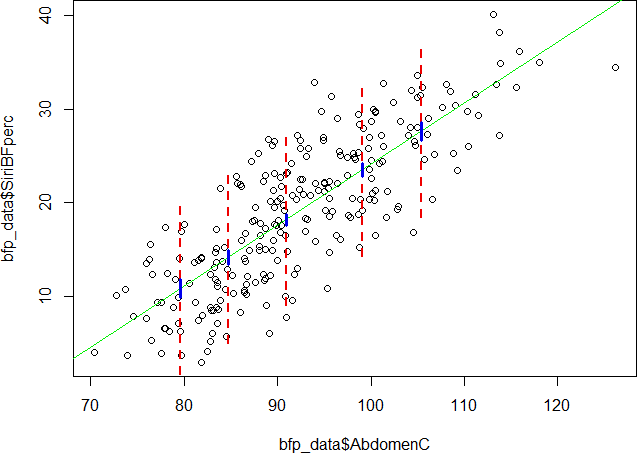
\includegraphics[width=\textwidth]{plot_with_intervals.png}
	\label{figure:ci_pi}
\end{figure}

\subsection*{Part C}

We then fitted a linear regression model with the predictors being: abdomen, neck, chest, hip, thigh, knee, ankle, bicep, forearm, and wrist circumferences, in addition to weight and height. This model will be referred to as the full model. Following this, we can compare the plots of residuals vs fitted values, residual Q-Q plots and perform a Shapiro-Wilk test for both models.

There are four assumptions that we make in linear regression that must be checked by examining the aforementioned plots and the Shaprio-Wilk tests:
\begin{itemize}
	\item The response and predictors have a linear relationship
	\item The errors are independent
	\item The errors are normally distributed
	\item The errors have equal variance
\end{itemize}

First is the examination of the residuals vs fitted values of each model. As can be seen in figure \ref{figure:residuals}, there does not seem to be a nonlinear trend in either plot, indicating that our first assumption is valid. Examining the spread of the residuals shows that the variance is relatively constant for the reduced model with exception of less than 10\% body fat. The full model, however appears to have significantly less variance for measurements over 30\% body fat. 

\begin{figure}[H]
	\centering
	\caption{Residual vs Fitted Values Plots}
	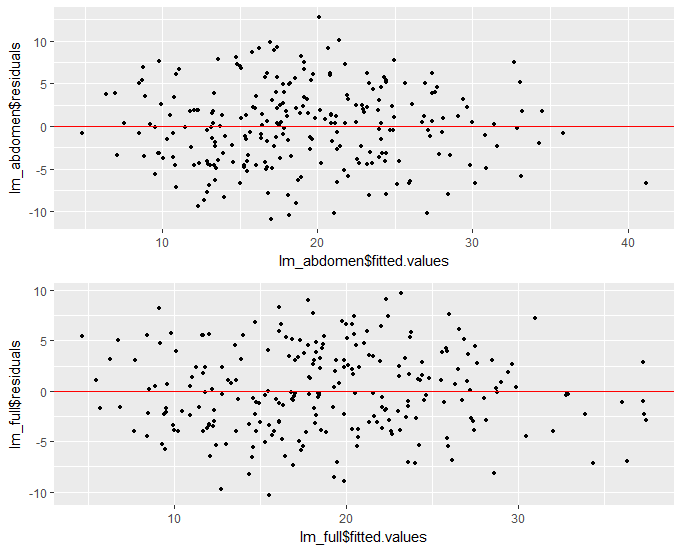
\includegraphics[width=\textwidth]{residuals_vs_fitted.png}
	\label{figure:residuals}
\end{figure}

Second, to determine the normality of the errors, the Q-Q plots of the residuals for each model are examined. The plot for the reduced model that follows shows a light tail on both ends, but is otherwise relatively normal.

\begin{figure}[H]
	\centering
	\caption{Reduced Model Q-Q Plot}
	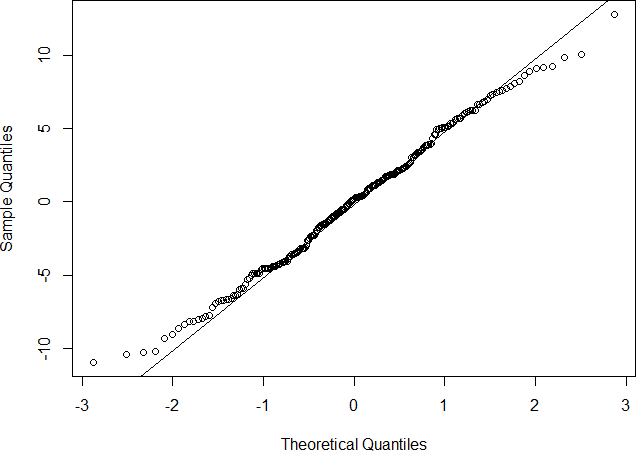
\includegraphics[width=\textwidth]{reduced_qq_plot.png}
\end{figure}

The Q-Q plot of the full model shows significantly lighter tails than the reduced model, but still does not appear to be skewed indicating that the distribution of the errors is mostly normal, with potential variance issues indicated by the tails.
\begin{figure}[H]
	\centering
	\caption{Full Model Q-Q Plot}
	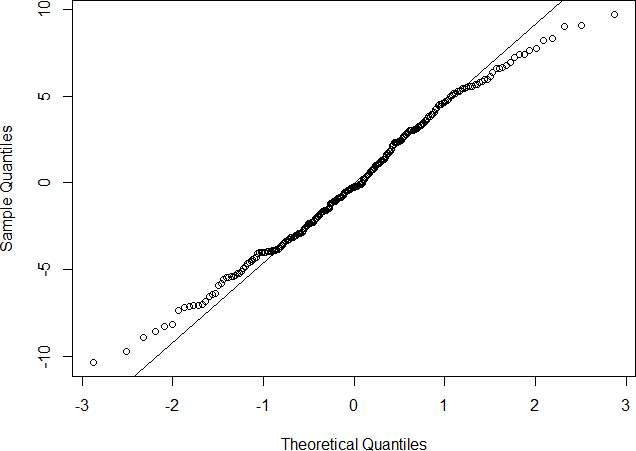
\includegraphics[width=\textwidth]{full_qq_plot.png}
\end{figure}

Next we perform a Shapiro-Wilk test on both models. This test is for the following hypotheses:
\vspace{-1cm}
\begin{center}
	\begin{align*}
		H_0&: \text{The errors are normally distributed}\\
		H_1&: \text{The errors are not normally distributed}
	\end{align*}
\end{center}

As we can see from the following table, the p-values for both models are significantly large enough to not reject the null hypothesis. This indicates that the errors are, in fact, normally distributed. It is worth noting that as we expected from the Q-Q plots, the reduced model has a higher p-value, meaning that the possibility for the errors being normal is higher.
\begin{table}[H]
	\centering
	\begin{tabular}{ r | c | c }
		& Full Model & Reduced Model \\ \hline
		W & 0.99087 & 0.99373 \\
		P & 0.1271 & 0.3954
	\end{tabular}
	\caption{Shapiro-Wilk Tests}
	\label{table:SW}
\end{table}

The final assumption -- that the errors must be independent -- is assumed to be true as the measurements were taken from a sample of the population. Also, logically, the likelihood of one person's body fat percentage affecting another person's seems improbable.

%%%%%%%%%%%%%%%%%%%%%%%%%%%%%%%%%%%%%%%%%%%%%%%%%%%%%%%%%%%%%%%%%%%%
%%% SECTION: CODE APPENDIX
%%%%%%%%%%%%%%%%%%%%%%%%%%%%%%%%%%%%%%%%%%%%%%%%%%%%%%%%%%%%%%%%%%%%

%\newpage
%\section*{R Code}
%\lstinputlisting[language=R]{../hw3.r}

\end{document}